% !Mode:: "TeX:UTF-8"

\chapter{末端授粉效率的提高}\label{ch:6}
\section{引言}

在自主授粉机器人系统中,机械臂末端的定位精度直接影响授粉成功率与任务效率。由于农业场景中目标花朵小巧、分布密集、易受遮挡,且常缺乏深度信息,导致传统依赖点云建模或模板匹配的定位方法在末端对准精度上存在显著不足。

为了解决这一问题,本文提出一种基于 Transformer 的机器臂授粉末端平移和旋转误差预测方法,仅利用 RGB 图像输入,通过深度学习直接预测末端与目标花朵之间的三维平移与旋转误差。该方法可实时修正末端位姿,显著提升授粉效率并缩短伺服时间。

\section{方法}

\subsection{末端误差建模}
\begin{figure}[htb]
	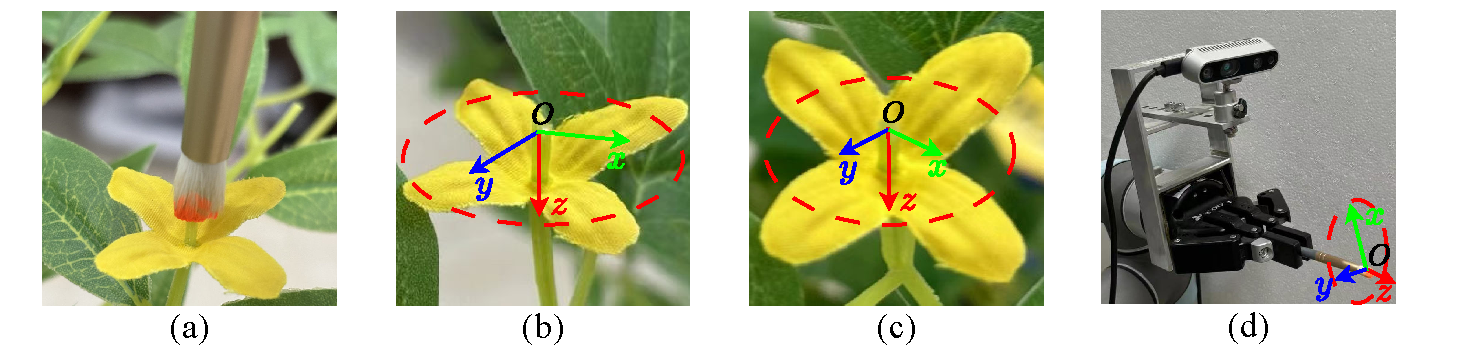
\includegraphics[width=1 \textwidth]{error}
	\caption[不同位置构建的笛卡尔坐标系]{不同位置构建的笛卡尔坐标系} % 中括号中内容为插图索引中显示内容,可在题注内容过长时使用
	\label{fig:effective1}
\end{figure}


为了描述平移偏差误差与姿态旋转偏差误差,需要分别在目标花朵与授粉机器人的末端构建两个笛卡尔坐标系,记为 $C_{A}$ 与 $C_{B}$。构建在花朵上的笛卡尔坐标系 $C_{A}$ 以柱头末端为原点 $O$,其 $x$ 轴与 $y$ 轴构成的平面与花瓣平面平行,$z$ 轴与柱头平行,指向花朵内部,如\cref{fig:effective1}中$b,c$ 所示。而构建在授粉机器人末端的笛卡尔坐标系 $C_{B}$,以刷头末端为原点 $O$,该坐标系通过对 UR5 机械臂的 TCP 坐标系进行平移获得,如图\cref{fig:effective1}中d 所示。$C_{A}$ 可以通过一个 $4\times4$ 的平移—旋转矩阵 $TR$ 从 $C_{B}$ 推导得到:
\begin{equation}
	\label{eq0_1}
	TR=
	\begin{bmatrix}
		R_{11} & R_{12} & R_{13} & t_{1} \\
		R_{21} & R_{22} & R_{23} & t_{2} \\
		R_{31} & R_{32} & R_{33} & t_{3} \\
		0 & 0 & 0 & 1 \\
	\end{bmatrix}
\end{equation}
\begin{equation}
	\label{eq0_2}
	C_{A} = TR\cdot C_{B}
\end{equation}

平移偏差误差与姿态旋转偏差误差分别为平移旋转矩阵 $TR$ 中的平移向量 $t$ 与由旋转矩阵 $R$ 推导出的旋转向量:
\begin{equation}
	\label{eq0_3}
	t = \begin{bmatrix}
		t_1  &	t_2 &	t_3
	\end{bmatrix}^\mathrm{T}
\end{equation}
\begin{equation}
	\label{eq0_4}
	R=
	\begin{bmatrix}
		R_{11} & R_{12} & R_{13}\\
		R_{21} & R_{22} & R_{23} \\
		R_{31} & R_{32} & R_{33} 
	\end{bmatrix}
\end{equation}


当授粉机器人末端处于理想授粉姿态时,平移偏差误差与旋转姿态偏差误差的数值趋近于零。此时,授粉机器人末端的刷头垂直于目标花朵的花瓣平面,恰好接触柱头,即坐标系 $C_{A}$ 与 $C_{B}$ 重合,如\cref{fig:effective1}中$a$ 所示。
\begin{equation}
	\label{eq0_4_1}
	\begin{split}
		\theta &= \cos^{-1}(\frac{trace(R) - 1}{2})\\
		\overrightarrow{V}&= \frac{1}{2\sin(\theta)}\begin{bmatrix}
			R_{32} - R_{23}\\
			R_{13} - R_{13} \\
			R_{21} - R_{12} 
		\end{bmatrix} \\
		\overrightarrow{W} &= \theta \overrightarrow{V}
	\end{split}
\end{equation}

模型预测的平移偏差误差与旋转姿态偏差误差分别记为 $\hat{t}$ 与 $\hat{R}$。末端执行器到目标花朵柱头之间的实际误差与预测误差之间的差值,分别作为平移误差($TE$)与旋转误差($RE$)进行计算。根据公式~(\ref{eq0_4_1}),旋转矩阵 $R$ 与 $\hat{R}$ 可被转换为旋转向量 $\overrightarrow{W}$ 与 $\hat{\overrightarrow{W}}$:
\begin{equation}
	\label{eq0_5}
	TE = \Vert \hat{t} -t \Vert \\
\end{equation}
\begin{equation}
	\label{eq0_6}
	RE = 1 -  \frac{\hat{\overrightarrow{W}}\overrightarrow{W}}{\Vert\hat{\overrightarrow{W}}\Vert\Vert\overrightarrow{W}\Vert}
\end{equation}

$TE$ 的单位为厘米(cm),表示预测平移误差与实际平移误差之间的空间距离;$RE$ 为无量纲量,表示预测旋转向量误差与实际旋转向量误差之间的余弦距离。

\subsection{基于Transformer的授粉末端误差估计网络}

为提高授粉机器人末端姿态估计的精度,本研究提出了一种基于Transformer的末端误差差估计网络。该网络以“手眼一体”RGB相机采集的图像作为输入,输出授粉末端相对于目标花朵在笛卡尔坐标系下的平移与旋转偏差向量 $(\Delta T_{x}, \Delta T_{y}, \Delta T_{z},\Delta W_{x}, \Delta W_{y}, \Delta W_{z})$,其中 $\Delta T$ 表示三维平移偏差,$\overrightarrow{W}$ 表示三维旋转向量偏差。


为了从图像中提取高质量的空间特征,模型采用了预训练的卷积神经网络作为特征提取模块。该网络能够有效捕捉图像中的空间层级信息,将原始图像转换为高维特征向量。随后,为保留图像的空间结构信息,模型在特征向量中引入了二维正弦位置编码,并将其与特征相加后输入至Transformer编码器中。

\begin{figure}[htb]
	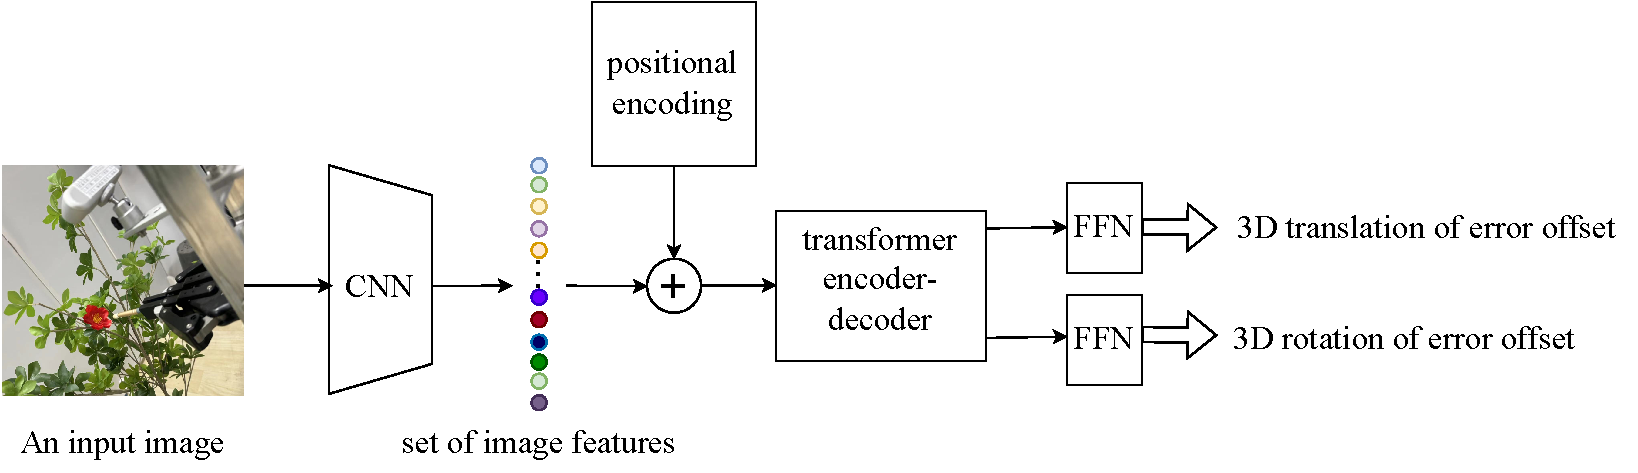
\includegraphics[width=1 \textwidth]{model}
	\caption[用于估计授粉末端平移和旋转误差的模型整体框架]{用于估计授粉末端平移和旋转误差的模型整体框架} % 中括号中内容为插图索引中显示内容,可在题注内容过长时使用
	\label{fig:effective3}
\end{figure}

\cref{fig:effective3} 展示了模型整体框架。首先,输入图像经过卷积神经网络(CNN)提取高维图像特征。随后,这些特征被加入位置编码后输入至 Transformer 模块中。Transformer 的输出特征分别由两个独立的前馈神经网络处理,用于分别预测平移偏差与旋转偏差。

在Transformer编码器中,采用了五头多头注意力机制以并行捕获不同子空间的信息。编码后的特征由解码器进一步处理,解码器通过查询机制将嵌入向量转换为用于预测的特征表示。最终,这些特征分别输入两个前馈神经网络中,分别用于回归平移偏差向量 $\Delta T$ 与旋转偏差向量 $\overrightarrow{W}$。

\begin{figure}[htb]
	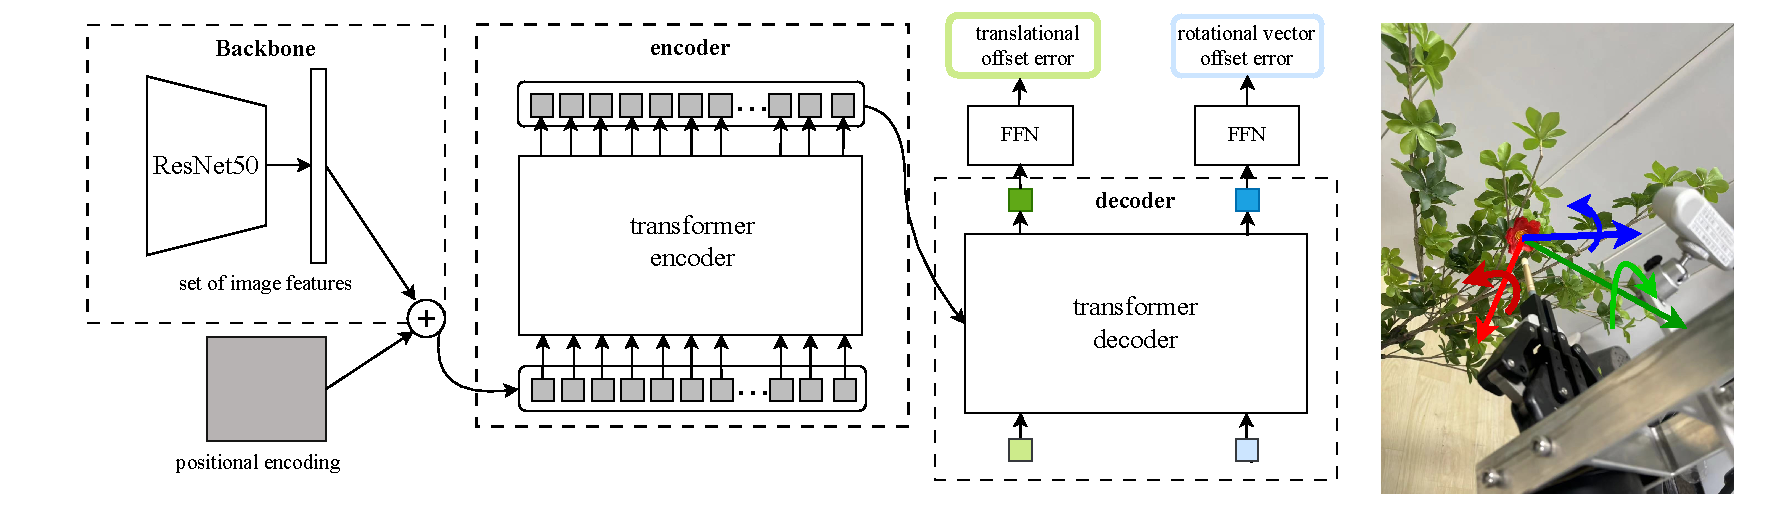
\includegraphics[width=1 \textwidth]{Architecture}
	\caption[用于估计授粉末端平移和旋转误差的模型结构]{用于估计授粉末端平移和旋转误差的模型结构
	} % 中括号中内容为插图索引中显示内容,可在题注内容过长时使用
	\label{fig:effective4}
\end{figure}
\cref{fig:effective4} 展示了完整网络结构,采用 ResNet50 作为主干网络,从输入图像中学习高层特征。这些特征随后与位置编码相结合,并输入至编码器中。随后,解码器首先输出一个用于预测平移偏差的特征向量,该向量作为输入传递给一个前馈神经网络进行平移偏差的回归预测。接着,该特征向量被用作查询输入,再次送入解码器,生成另一个特征向量,并由另一个独立的前馈神经网络用于旋转姿态偏差的预测。




\subsection{损失函数设计}
在本章所提出的模型中,分别对平移偏差误差与旋转姿态偏差误差进行预测,因此设计了两个独立的损失函数。第一个损失函数记为 $Loss_{T}$,用于度量模型所预测的授粉机器人末端相对于目标花朵柱头的空间位置偏差误差与实际空间偏差误差之间的均方差。$Loss_{T}$ 定义如下:
\begin{equation}
	\label{eq5}
	Loss_{T} = \frac{1}{2m}\sum\limits_{x\in\mathcal{M}}(\hat{T_{n}} - T_{n})^{2} 
\end{equation}

其中,$\mathcal{M}$ 表示测试数据集的集合,$m$ 为集合中的样本数,$\hat{T_{n}}$ 与 $T_{n}$ 分别表示模型预测的平移偏差误差与真实平移偏差误差。

第二个损失函数记为 $Loss_{R}$,用于衡量模型所预测的授粉机器人末端相对于目标柱头的空间旋转误差与实际旋转误差之间的差异。$Loss_{R}$ 定义如下:
\begin{equation}
	\label{eq6}
	Loss_{R} = \frac{1}{2m}\sum\limits_{x\in\mathcal{M}}(\frac{1}{\sigma_{1}^{2}}(\Vert\hat{\theta} -\theta \Vert^{2}) + \frac{1}{\sigma_{2}^{2}}(1 - \frac{\hat{\overrightarrow{V}}\overrightarrow{V}}{\Vert\hat{\overrightarrow{V}}\Vert\Vert\overrightarrow{V}\Vert}) + \log(\sigma_{1}\sigma_{2})) 
\end{equation}

其中,$\mathcal{M}$ 表示测试数据集的集合,$m$ 为集合中的样本数。变量 $\hat{\theta}$、$\theta$、$\hat{\overrightarrow{V}}$ 和 $\overrightarrow{V}$ 分别表示预测与真实旋转角度和旋转轴,$\sigma_{1}$ 与 $\sigma_{2}$ 为需要通过训练学习的可调参数。

最终用于模型训练的联合损失函数定义如下:
\begin{equation}
	\label{eq7}
	Loss =  \alpha Loss_{T} + \beta Loss_{R}
\end{equation}

该合损失函数综合衡量模型在训练过程中对平移偏差误差与旋转姿态偏差误差的拟合能力。其中,$\alpha$ 与 $\beta$ 为可调超参数,分别表示平移损失与旋转损失的加权系数,需在模型训练过程中进行系统性调整以获得最优性能。


\section{实验设计与分析}

\subsection{数据预处理}
\begin{figure}[htb]
	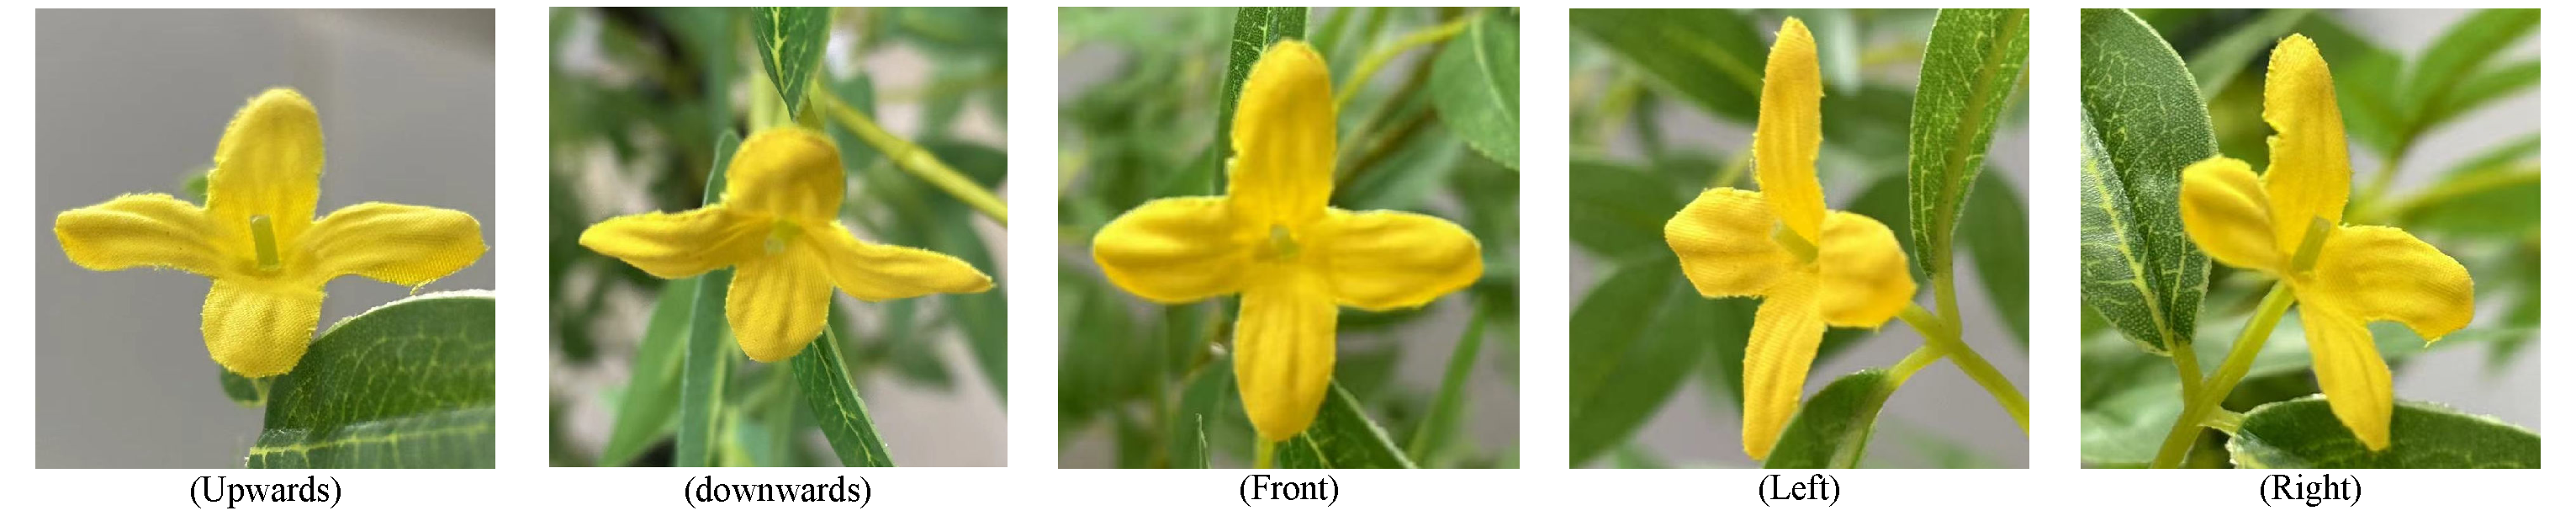
\includegraphics[width=1 \textwidth]{direct_flower}
	\caption[花朵相对于机械臂末端的不同方向姿态示意图]{花朵相对于机械臂末端的不同方向姿态示意图} % 中括号中内容为插图索引中显示内容,可在题注内容过长时使用
	\label{fig:effective_r_1}
\end{figure}
本实验所使用的图像数据均来源于自建授粉图像数据集,数据集中包含了由安装在机械臂上的相机在授粉过程中拍摄的图像,每张图像唯一对应一个待授粉花朵的姿态状态。如\cref{fig:effective_r_1}所示,依据花朵相对于机械臂末端的方向性特征,图像样本被划分为五类:左(L)、右(R)、上(U)、下(D)和正前方(F)。详细的统计信息如表\cref{tab:effective_r_1}所示。




\begin{table}[htbp]
	\centering
	\caption[数据集中不同方向花朵图像的数量统计]{数据集中不同方向花朵图像的数量统计}
	\begin{tabularx}{\textwidth}{YYY}
		\toprule
		\textbf{方向} & \textbf{图像数量} & \textbf{占比(\%)} \\
		\midrule
		L & 261 & 20.6 \\
		R & 274 & 21.7 \\
		F & 230 & 18.2 \\
		U & 256 & 20.3 \\
		D & 243 & 19.2 \\
		\bottomrule
	\end{tabularx}
	\label{tab:effective_r_1}
	
	\vspace{1mm}
	\noindent{\footnotesize 其中 “F”、“L”、“R”、“U” 和 “D” 分别表示前方、左侧、右侧、上方与下方。}
\end{table}


为保证模型输入数据的一致性,首先将机械臂末端相机采集的所有图像统一调整为 $(224 \times 224)$ 的分辨率。随后,对图像进行了归一化处理,将像素值缩放至 $[0, 1]$ 区间,以提升模型训练的稳定性。此外,为增强数据多样性并缓解过拟合问题,应用了包括缩放、裁剪和色彩变换等在内的数据增强策略。

在标签数据方面,假设位置偏差为 $\Delta T = (\Delta T_{x}, \Delta T_{y}, \Delta T_{z})$,旋转偏差为 $\Delta \overrightarrow{W} = (\Delta W_{x}, \Delta W_{y}, \Delta W_{z})$,其中 $||\Delta T|| < D$,$D$ 为常数。根据式~(\ref{eq1}) 和式~(\ref{eq2}) 对平移与旋转误差进行了归一化与缩放处理,使其值域限制在 $[-1, 1]$ 区间内,处理过程如下:

\begin{equation}
	\label{eq1}
	\Delta T_{n} = \frac{\Delta T}{D}
\end{equation}
\begin{equation}
	\label{eq2}
	\overrightarrow{W} = \theta\overrightarrow{V}
\end{equation}
\begin{equation}
	\label{eq3}
	\theta = \sqrt{\Delta W_{x}^{2} + \Delta W_{y}^{2} + \Delta W_{z}^{2}}
\end{equation}
\begin{equation}
	\label{eq4}
	\overrightarrow{V} = \left(\frac{\Delta W_{x}}{\theta},\frac{\Delta W_{y}}{\theta},\frac{\Delta W_{z}}{\theta}\right)
\end{equation}

符号 $\theta$ 在公式\cref{eq3} 中表示旋转角度,$\overrightarrow{V}$ 表示旋转轴方向的单位向量。归一化后的标签数据为 $(\Delta T_{n}, \overrightarrow{V}, \frac{\theta}{2\pi})$。



\subsection{训练细节}

本模型的训练在配备 NVIDIA V100 GPU 的计算环境中进行。优化器采用 Adam 方法,初始学习率设置为 0.01,并使用学习率衰减策略,随着训练过程的推进,学习率逐步降低至 0.00001。训练过程中采用自定义的损失函数(见公式~(\ref{eq7}))。在训练中,损失函数中的超参数 $\alpha$ 与 $\beta$ 会显著影响模型的收敛性能。经过多轮实验验证,最终选定 $\alpha = 0.0025$,$\beta = 1$,该设置有助于模型更稳定地收敛。

在数据划分方面,所有具有不同方向姿态的花朵图像被随机打乱后划分为10个子集,并采用K折交叉验证的方式进行训练。每轮训练选择其中一个子集作为测试集,其余九个作为训练集,总共进行10轮。模型在训练初期收敛迅速,后期趋于稳定。\cref{fig:effective_r_3} 展示了训练过程中损失值、平移误差($TE$)以及旋转误差($RE$)的变化趋势。

\begin{figure}[htb]
	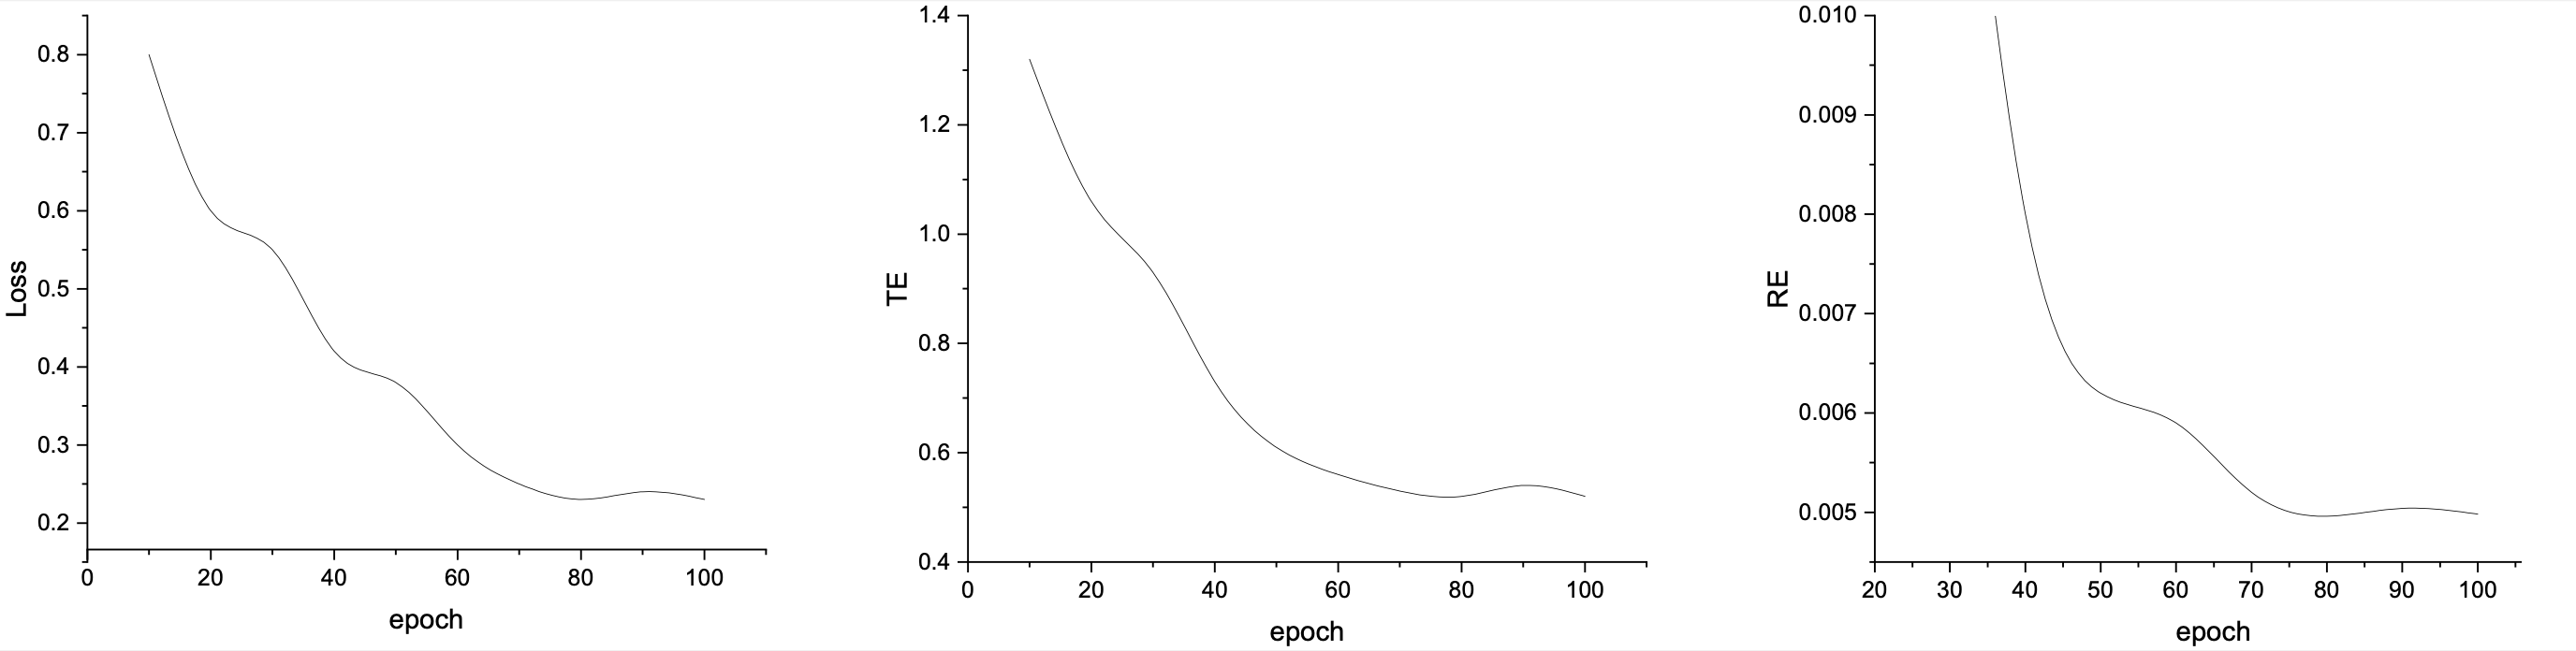
\includegraphics[width=1 \textwidth]{train.png}
	\caption[模型训练过程中的变化曲线]{模型训练过程中损失值(Loss)、平移误差($TE$)与旋转误差($RE$)的变化曲线} % 中括号中内容为插图索引中显示内容,可在题注内容过长时使用
	\label{fig:effective_r_3}
\end{figure}




\subsection{实验结果与分析}

本节重点比较本章所提出方法与没有引入本章所提出方法在机器人末端授粉准确性上的差异,特别是在授粉机器人末端执行器精度与单花授粉效率方面的改进。

我们针对不同方向姿态的花朵进行了分组实验,评估模型的平移与旋转偏差预测精度及检测速度。实验结果表明,不同方向的花朵在预测效果上存在轻微差异。如\cref{tab:effective_r_3} 和\cref{fig:effective_r_4} 所示,朝前方向的花朵具有最小的平移与旋转误差,表现最佳,其次为朝上方向;左右方向由于环境对称性,预测误差几乎一致;而朝下方向的误差最大。但无论方向如何,模型的检测速度(FPS)基本保持稳定。




\begin{table}[htbp]
	\centering
	\caption[模型在不同方向上花朵的实验结果]{模型在不同方向上花朵的实验结果}
	\begin{tabularx}{\textwidth}{YYYY}
		\toprule
		\textbf{方向} & \textbf{平移误差 TE} & \textbf{旋转误差 RE} & \textbf{检测速度 FPS} \\
		\midrule
		L & 0.82 & 0.0049 & 41 \\
		R & 0.82 & 0.0049 & 42 \\
		F & 0.78 & 0.0047 & 43 \\
		U & 0.80 & 0.0048 & 42 \\
		D & 0.87 & 0.0051 & 41 \\
		\bottomrule
	\end{tabularx}
	\label{tab:effective_r_3}
	\noindent{\footnotesize{方向 “F”、 “L”、 “R”、 “U” 和 “D” 分别表示前方、左侧、右侧、上方与下方。}}
\end{table}

\begin{figure}[htb]
	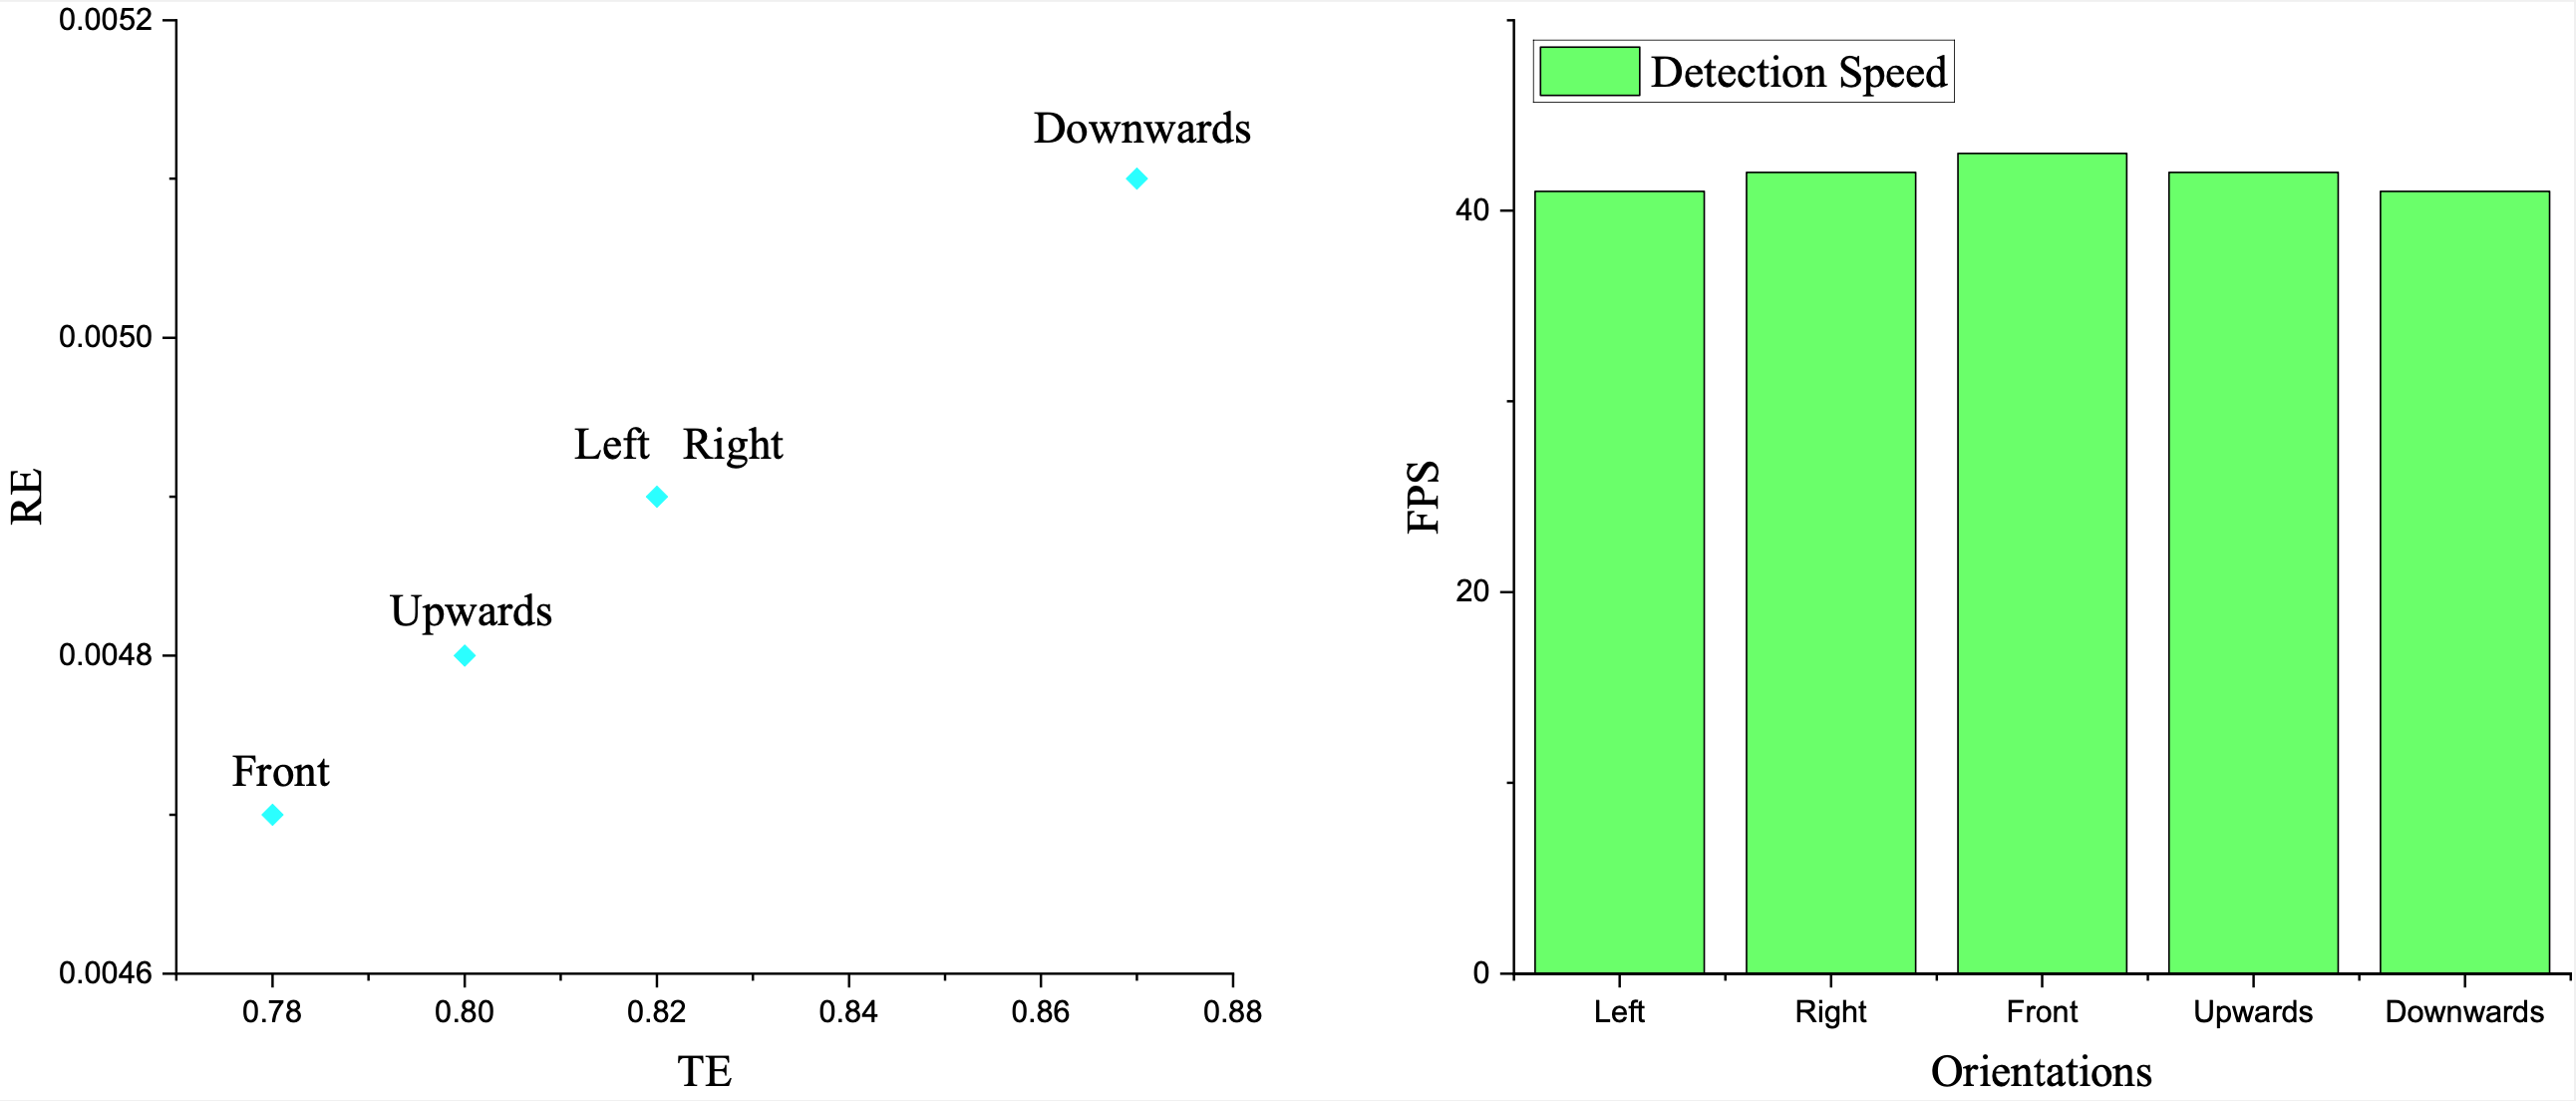
\includegraphics[width=1 \textwidth]{direct.png}
	\caption[模型在不同方向花朵上预测的平移和旋转误差]{模型在不同方向花朵上预测的平移和旋转误差} % 中括号中内容为插图索引中显示内容,可在题注内容过长时使用
	\label{fig:effective_r_4}
\end{figure}

本实验使用前述授粉机器人作为实验平台。机器人完成一次授粉共包含五个步骤,在第四步后其末端执行器相对目标柱头的定位误差为 1.5 cm。在此基础上,我们新增了“精调定位”步骤,输入图像至训练好的模型中,预测平移与旋转偏差,并对授粉末端姿态进行调整。

如\cref{tab:effective_r_4} 所示,加入该“精调定位”步骤后,授粉末端与目标之间的误差显著缩小,为后续伺服授粉步骤减少了搜索范围。实验显示,伺服过程时间从12.7秒缩短至3.1秒,平均成功率达到86.19\%,授粉成功率保持一致。\cref{tab:effective_r_5} 显示我们方法将末端平均定位误差缩小至0.81 cm,精度提升达46.67\%,旋转误差为0.0049,平均单花授粉效率提升达50.9\%。

\begin{table}[htbp]
	\centering
	\caption[本方法引入前后授粉系统各步骤平均耗时比较]{本方法引入前后授粉系统各步骤平均耗时比较}
	\begin{tabularx}{\textwidth}{YYY}
		\toprule
		\textbf{步骤}	& \textbf{baseline 耗时(秒)}	& \textbf{本方法耗时(秒)}     \\
		\midrule
		花朵检测	& 0.0928			& 0.0927		\\
		柱头识别   & 0.025			& 0.024			\\
		位置计算(含运动)    & 1.8			& 1.8			\\
		接近花朵(含运动)   & 4.2			& 4.2			\\
		\textcolor{red}{精调定位}   & /			& 0.024			\\
		伺服授粉(含运动)   & 12.7			& \textcolor{red}{3.1}			\\
		\bottomrule
	\end{tabularx}
	\label{tab:effective_r_4}
	
	\noindent{\footnotesize{“精调定位"步骤是一个额外步骤。增加这一步骤,“伺服”步骤所花费的时间就会大大减少,只需 3.1 秒就能达到相同的授粉成功率。}}
\end{table}
\begin{table}[H]
	\centering
	\caption[本方法与对照方法在不同方向花朵上的误差与耗时对比]{本方法与对照方法在不同方向花朵上的误差与耗时对比}
	\begin{tabularx}{\textwidth}{YYYYY}
		\toprule
		\textbf{方向}	& \textbf{方法}	& \textbf{TE}     & \textbf{RE} & \textbf{耗时(秒)}\\
		\midrule
		\multirow{2}{*}{L}	& baseline			& 1.53			& / & 18.78\\
		& 本方法			& 0.82			& 0.0050 & 9.22\\
		\midrule
		\multirow{2}{*}{R}    & baseline			& 1.52			& / & 18.80\\
		& 本方法			& 0.82			& 0.0050 & 9.23\\
		\midrule
		\multirow{2}{*}{F}    & baseline			& 1.48			& / & 18.85\\
		& 本方法			& 0.80			& 0.0048 & 9.22\\
		\midrule
		\multirow{2}{*}{U}   & baseline			& 1.53			& / & 18.79\\
		& 本方法			& 0.81			& 0.0049 & 9.24\\
		\midrule
		\multirow{2}{*}{D}   & baseline			& 1.55			& / & 18.83\\
		& 本方法			& 0.83			& 0.0052 & 9.26\\
		\bottomrule
	\end{tabularx}
	\label{tab:effective_r_5}
	\noindent{\footnotesize{方向“F”、“L”、“R”、“U”与“D”分别代表前、左、右、上与下。没有引入本章方法的授粉机器人为对照方法。}}
\end{table}
\subsection{消融实验}
\begin{table}[htbp]
	\centering
	\caption[不同主干网络结构与位置编码对模型预测平移与旋转误差精度的影响]{不同主干网络结构与位置编码对模型预测平移与旋转误差精度的影响}
	\begin{tabularx}{\textwidth}{YYYY}
		\toprule
		\textbf{主干网络} & \textbf{位置编码} & \textbf{TE(cm)} & \textbf{RE} \\
		\midrule
		\multirow{2}{*}{ResNet50} & \ding{51} & 0.81 & 0.0049 \\
		& \ding{55} & 1.19 & 0.0051 \\
		\midrule
		\multirow{2}{*}{ResNet18} & \ding{51} & 0.92 & 0.0053 \\
		& \ding{55} & 1.33 & 0.0054 \\
		\midrule
		\multirow{2}{*}{ResNet101} & \ding{51} & 0.86 & 0.0050 \\
		& \ding{55} & 1.21 & 0.0050 \\
		\midrule
		\multirow{2}{*}{VGG16} & \ding{51} & 0.96 & 0.0053 \\
		& \ding{55} & 1.32 & 0.0055 \\
		\midrule
		\multirow{2}{*}{VGG19} & \ding{51} & 0.99 & 0.0054 \\
		& \ding{55} & 1.33 & 0.0055 \\
		\midrule
		\multirow{2}{*}{DenseNet-121} & \ding{51} & 0.92 & 0.0054 \\
		& \ding{55} & 1.23 & 0.0055 \\
		\midrule
		\multirow{2}{*}{DenseNet-201} & \ding{51} & 1.10 & 0.0055 \\
		& \ding{55} & 1.38 & 0.0057 \\
		\bottomrule
	\end{tabularx}
	\label{tab:effective_r_6}
	\noindent{\footnotesize{表中 \ding{51} 表示该模型使用了位置编码,\ding{55} 表示未使用位置编码。}}
\end{table}
\begin{figure}[H]
	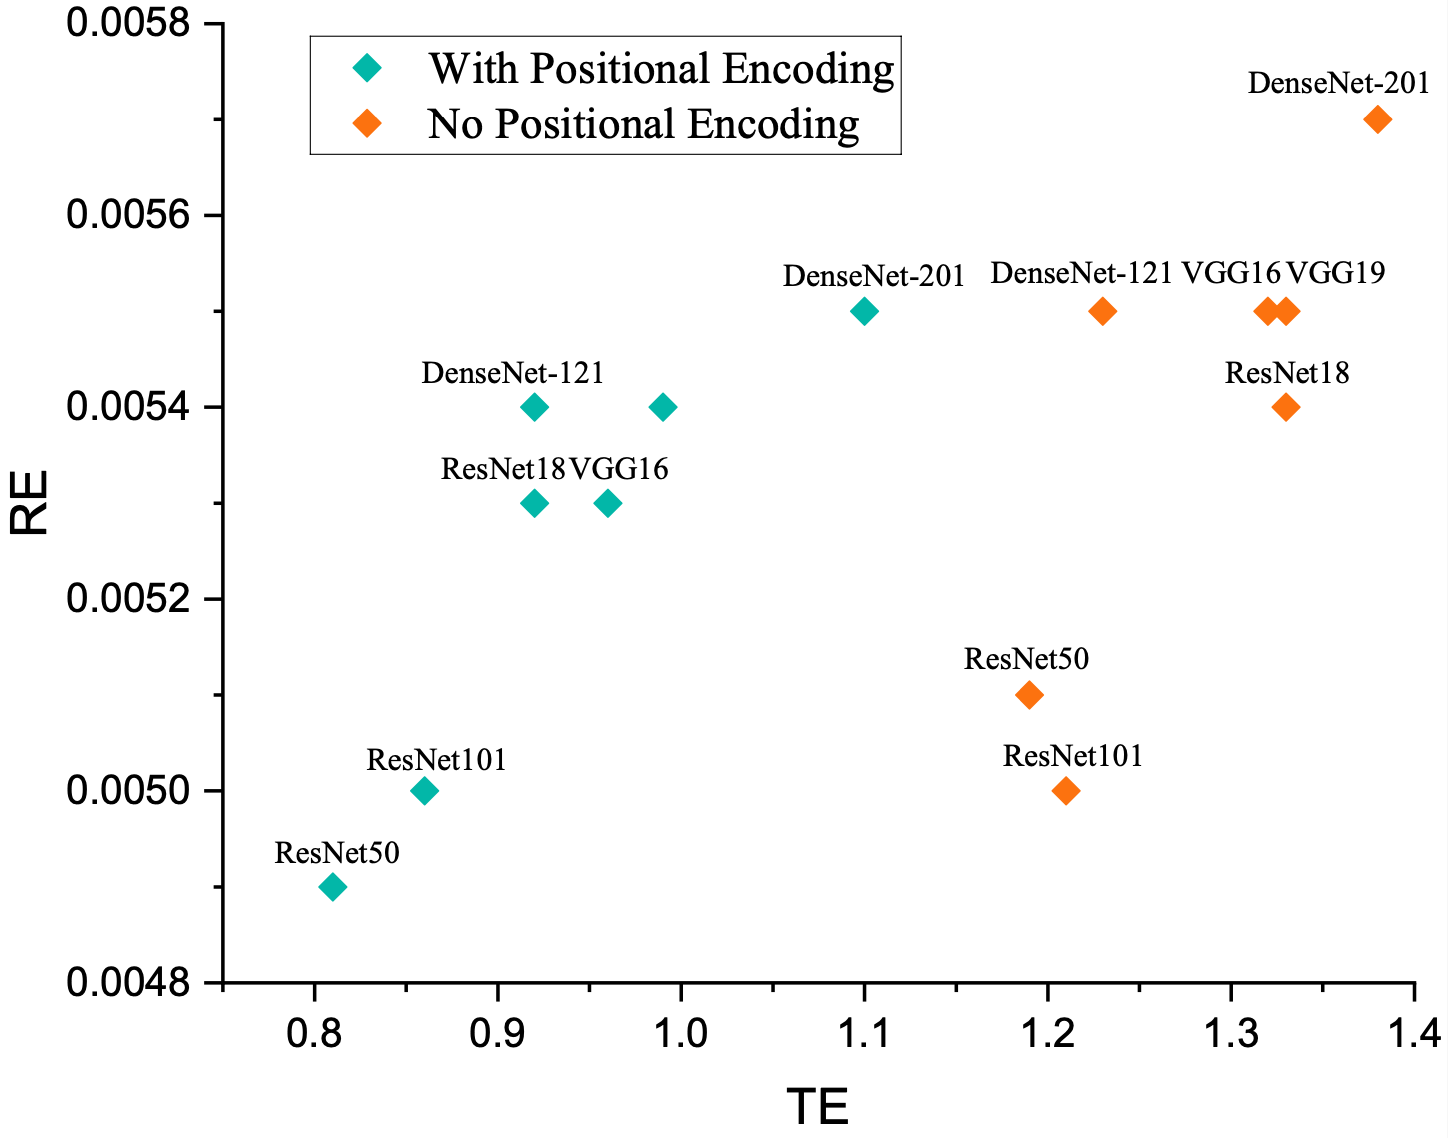
\includegraphics[width=0.6 \textwidth]{result.png}
	\caption[不同主干网络在是否加入位置编码条件下的平移误差]{不同主干网络在是否加入位置编码条件下的平移误差} % 中括号中内容为插图索引中显示内容,可在题注内容过长时使用
	\label{fig:effective_r_5}
\end{figure}
本研究开展了多组消融实验,以验证不同主干网络结构(Backbone)及位置编码的引入对模型平移偏差误差与旋转姿态偏差误差预测精度的影响。我们选取 ResNet50、ResNet18、ResNet101、VGG16、VGG19\cite{simonyan2014very}、DenseNet-121 与 DenseNet-201\cite{huang2017densely} 作为特征提取主干网络,并在每个主干结构下分别进行了添加与不添加位置编码的对比实验。

实验结果如\cref{tab:effective_r_6} 和\cref{fig:effective_r_5}所示,主干网络结构的选择及是否引入位置编码对模型的最终预测精度具有显著影响。其中,采用 ResNet50 作为主干网络并引入位置编码的模型在平移偏差与旋转姿态偏差预测中表现最优,分别达到 0.81 cm 与 0.0049 的误差。



\section{本章小节}

本章提出了一种基于 Transformer 的方法,实现了仅依赖 RGB 图像信息,对授粉机器人末端与目标授粉位置之间的平移误差与旋转姿态误差的端到端预测。实验结果表明,该方法能够有效地将末端执行器的定位误差控制在一定范围内,从而提升了整体的授粉作业效率。

在实验过程中,我们发现所提出的方法在面对不同方向的花朵时预测结果存在轻微差异,尤其是在处理朝下方向的花朵时,平移与旋转误差略有增大。这可能与机器人相机的观察角度相对于花朵方向的关系有关,使得特定姿态下的花朵识别与定位更困难。此外,实验还表明,引入位置编码的模型版本在平移与旋转误差预测方面表现更优,不同主干网络的特征提取能力也对模型性能具有显著影响。

尽管本方法在提升定位精度方面表现出良好的效果,但仍存在一些局限性:(1)本研究所使用的数据集为特定实验环境下采集,模型在多样化环境及不同种类花朵上的泛化能力仍需进一步验证;(2)在光照条件变化较大或存在遮挡的实际农田环境中,模型的鲁棒性可能受到一定影响,从而降低其预测性能。

上述问题提示我们,在未来的研究中仍需进一步优化模型结构与训练策略,以提升其在复杂农业场景中的适应性与可靠性,为实际部署提供坚实基础。




